\chapter{Event Reconstruction}\label{ch:event-reconstruction}
Events are reconstructed using a wide variety of algorithms designed to identify the products of collisions at the center of the detector. The algorithms transform the raw data read out from the detector -- hits in the inner detector silicon layers and TRT straws, energy deposits in calorimeter cells, and hits in the muon stations -- into a list of physics objects and their energies or momenta. This section describes the techniques used to identify the objects used in the analyses described in chapters~\ref{ch:model-independent-trilepton-search} and \ref{ch:trilepton-resonance-search}. 


\section{Electrons}\label{sec:event-reconstruction-electrons}
The signature of an electron is an energy deposit in the electromagnetic LAr calorimeter and a track reconstructed by the inner detector pointing at the calorimeter energy cluster.  The electron reconstruction algorithm begins by searching for clusters of energy in the calorimeter, based on a grid of $N_{\eta}\times N_{\phi}=200\times256$ towers of size $\Delta\eta\times\Delta\phi = 0.025\times0.025$. The tower energy is the sum of the cell energies in all longitudinal layers within the tower. Energy deposits with $\Et>2.5 \GeV$ within a $3\times 5$ window of towers form the seeds for both electrons and photons.

After passing loose shower shape requirements, the electron reconstruction algorithm searches for a track within a cone of radius $\Delta R=0.3$ around the cluster barycenter. Two hypotheses are used for track pattern recognition and fitting: the standard pion hypothesis, and an electron hypothesis that allows for larger energy losses due to bremsstrahlung. The cluster and track are required to satisfy one of the following two criteria:

\begin{itemize}
	\item The barycenter of the cluster and the track extrapolation to the middle layer of the LAr calorimeter satisfy $\Delta\phi<0.2$ in the direction of track bending or $\Delta\phi<0.05$ in the other direction. 
	\item The barycenter of the cluster and the track extrapolation to the middle layer of the LAr calorimeter, after rescaling the track momentum to the energy of the cluster, satisfy $\Delta\phi<0.1$ in the direction of track bending or $\Delta\phi<0.05$ in the other direction. 
\end{itemize}
 
For tracks with at least four silicon hits, the track and the cluster must also satisfy $|\Delta\eta|<0.05$. Finally, the cluster and track are rebuilt using algorithms optimized for measurement of the electron properties. The cluster is rebuilt sequentially in all four layers, using an area of $3\times7$ layer-2 cells in the barrel or $5\times5$ layer-2 cells in the end-caps. The tracks of electron candidates are refit using an optimized electron track filter based on the Gaussian Sum Filter (GSF) algorithm~\cite{gsf}. The GSF track and the cluster must satisfy tighter spatial matching criteria: $\Delta\phi<0.1$ in the direction of track bending, or $\Delta\phi<0.05$ in the opposite direction. GSF tracks with less than four silicon hits are required to satisfy even tighter criteria: $|\Delta\eta|<0.35$ or $0.2$ in the TRT barrel or end-cap, and $\Delta\phi<0.03$ in the direction of track bending or $\Delta\phi<0.02$ in the other direction. 

\subsection{Identification}
Further requirements can be imposed on electron candidates to suppress backgrounds from sources like misidentified hadronic jets, photon conversions, and electrons from hadron decays. Three increasingly stringent sets of cuts are defined, called loose, medium, and tight\footnote{An alternative method of identification using a likelihood-based multivariate method has been developed, but is not used in this dissertation}. The analyses described in chapters~\ref{ch:model-independent} and \ref{ch:resonance} use the tight cuts to select signal electrons, and the medium and loose cuts to derive data-driven background estimates. The loose set of cuts impose requirements on the shower shape in the first and second calorimeter layers, the quality of the track, the fraction of energy in hadronic calorimeter cells behind the LAr cells, and the spatial match of the track and the calorimeter cluster. The medium set of cuts consist of more stringent versions of the loose cuts, and additionally require a small track impact parameter with respect to the primary vertex, a minimum number of high-threshold TRT hits associated with the track, and a hit in the innermost pixel layer. The tight set of cuts again consist of more stringent versions of the medium cuts, with an additional cut on the ratio of the cluster energy to the track momentum ($E/p$) and a veto of candidates associated to a photon conversion vertex. 

\textcolor{red}{Consider putting a table in instead of a block of text.}

\subsection{Efficiency Measurements}\label{sec:reco-electron-efficiency}
The efficiency to detect an electron can be factorized into several components. The efficiency to detect a cluster in the electromagnetic calorimeter is very high, above $99\%$ for electrons with $\Et=15 \GeV$ and $99.9\%$ for $\Et=45 \GeV$. The reconstruction efficiency, covering the matching of a good-quality track to the cluster, and the identification efficiencies, covering the identification cuts with respect to reconstructed electrons, are measured using tag-and-probe techniques targeting $Z\rightarrow ee$ and $J/\Psi\rightarrow ee$ events~\cite{TheATLASCollaboration:2014vz}. One electron, the tag, is required to satisfy strict selection criteria, while the second electron, the probe, is used for efficiency measurements. The combined reconstruction and identification efficiencies are shown in figure~\ref{fig:electron-id-efficiencies}. The reconstruction efficiency makes up $1-5\%$ of the efficiency loss for electrons with $\Et<20 \GeV$, and less than $1\%$ for electrons with $\Et>80 \GeV$. The efficiencies are computed for both data and simulation, and the ratio between the two is used to correct the efficiency in simulation.

\begin{figure}[htbp]
	\centering
	\subfloat[] {
		\resizebox{0.45\textwidth}{!}{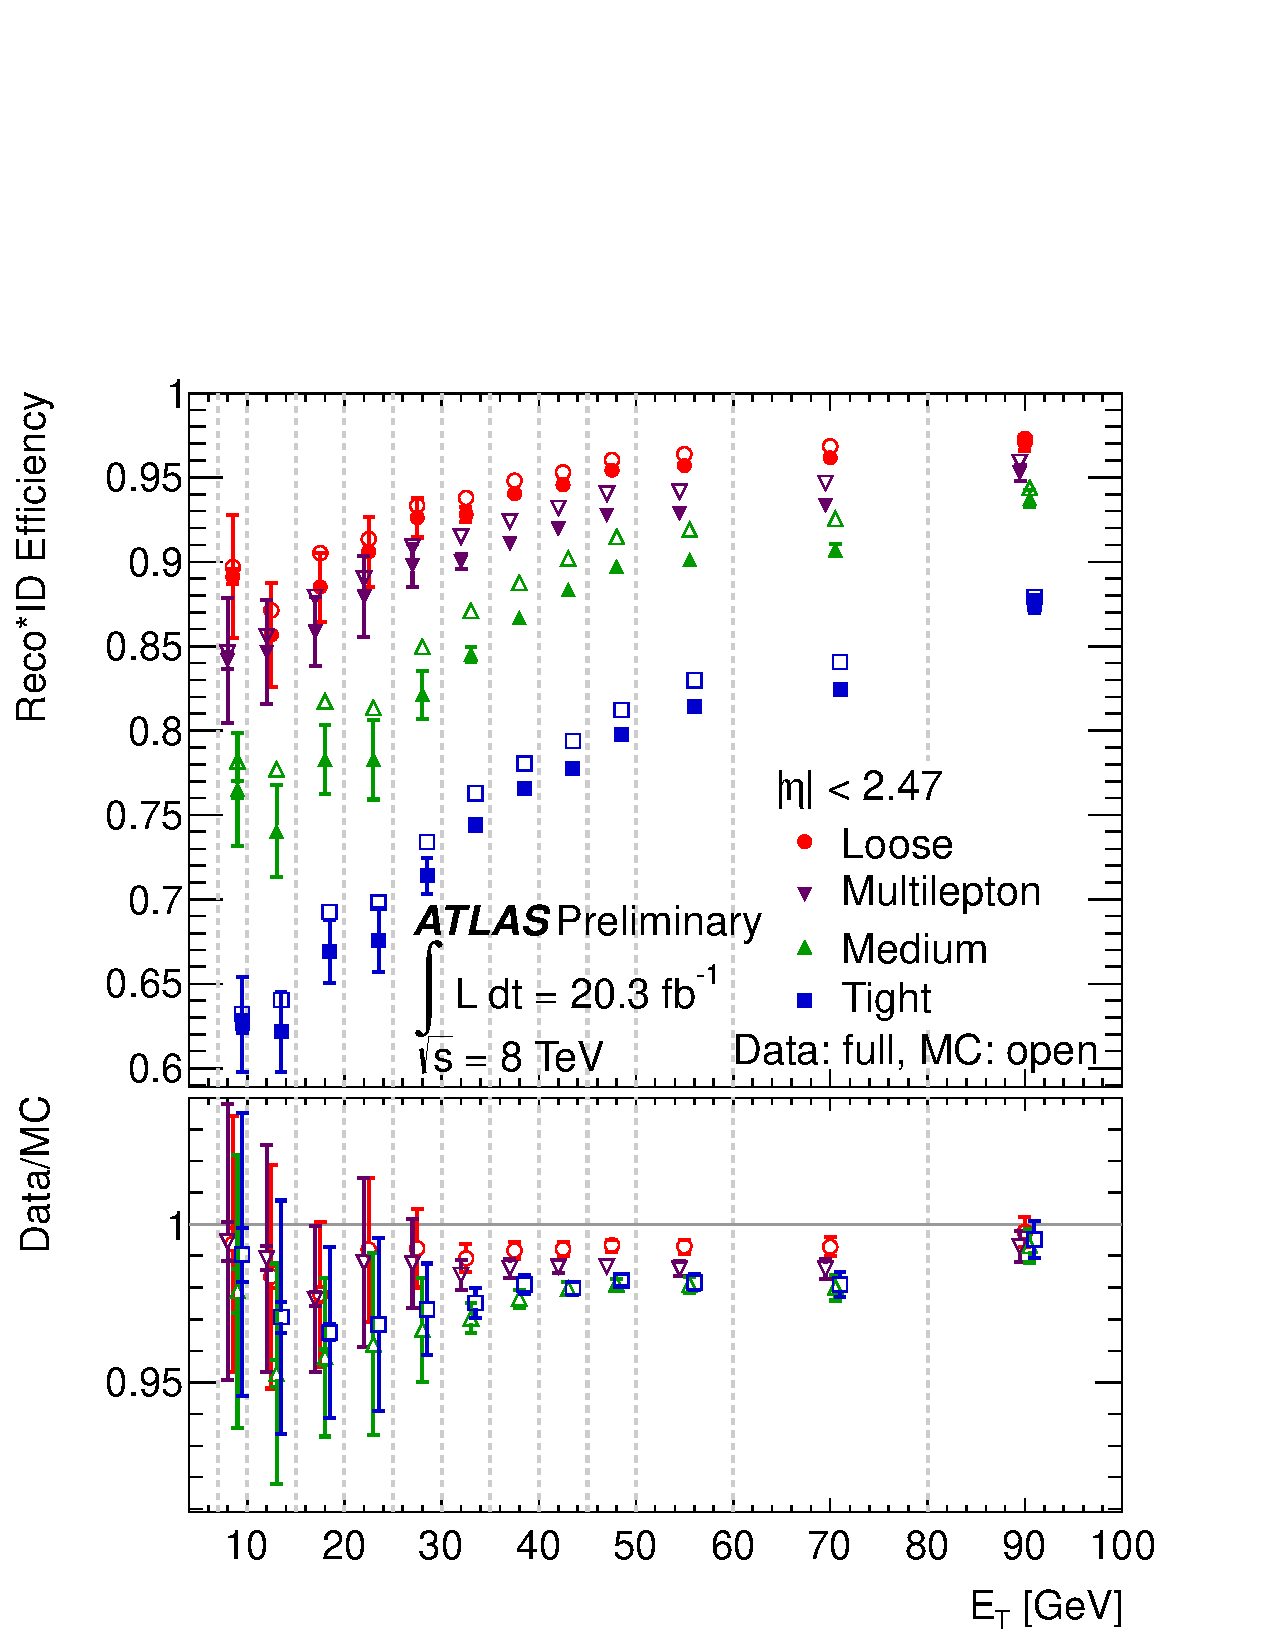
\includegraphics{figures/ch5-reconstruction/el_eff_idplusreco_ET}}
	}
	\hfill
	\subfloat[] {
		\resizebox{0.45\textwidth}{!}{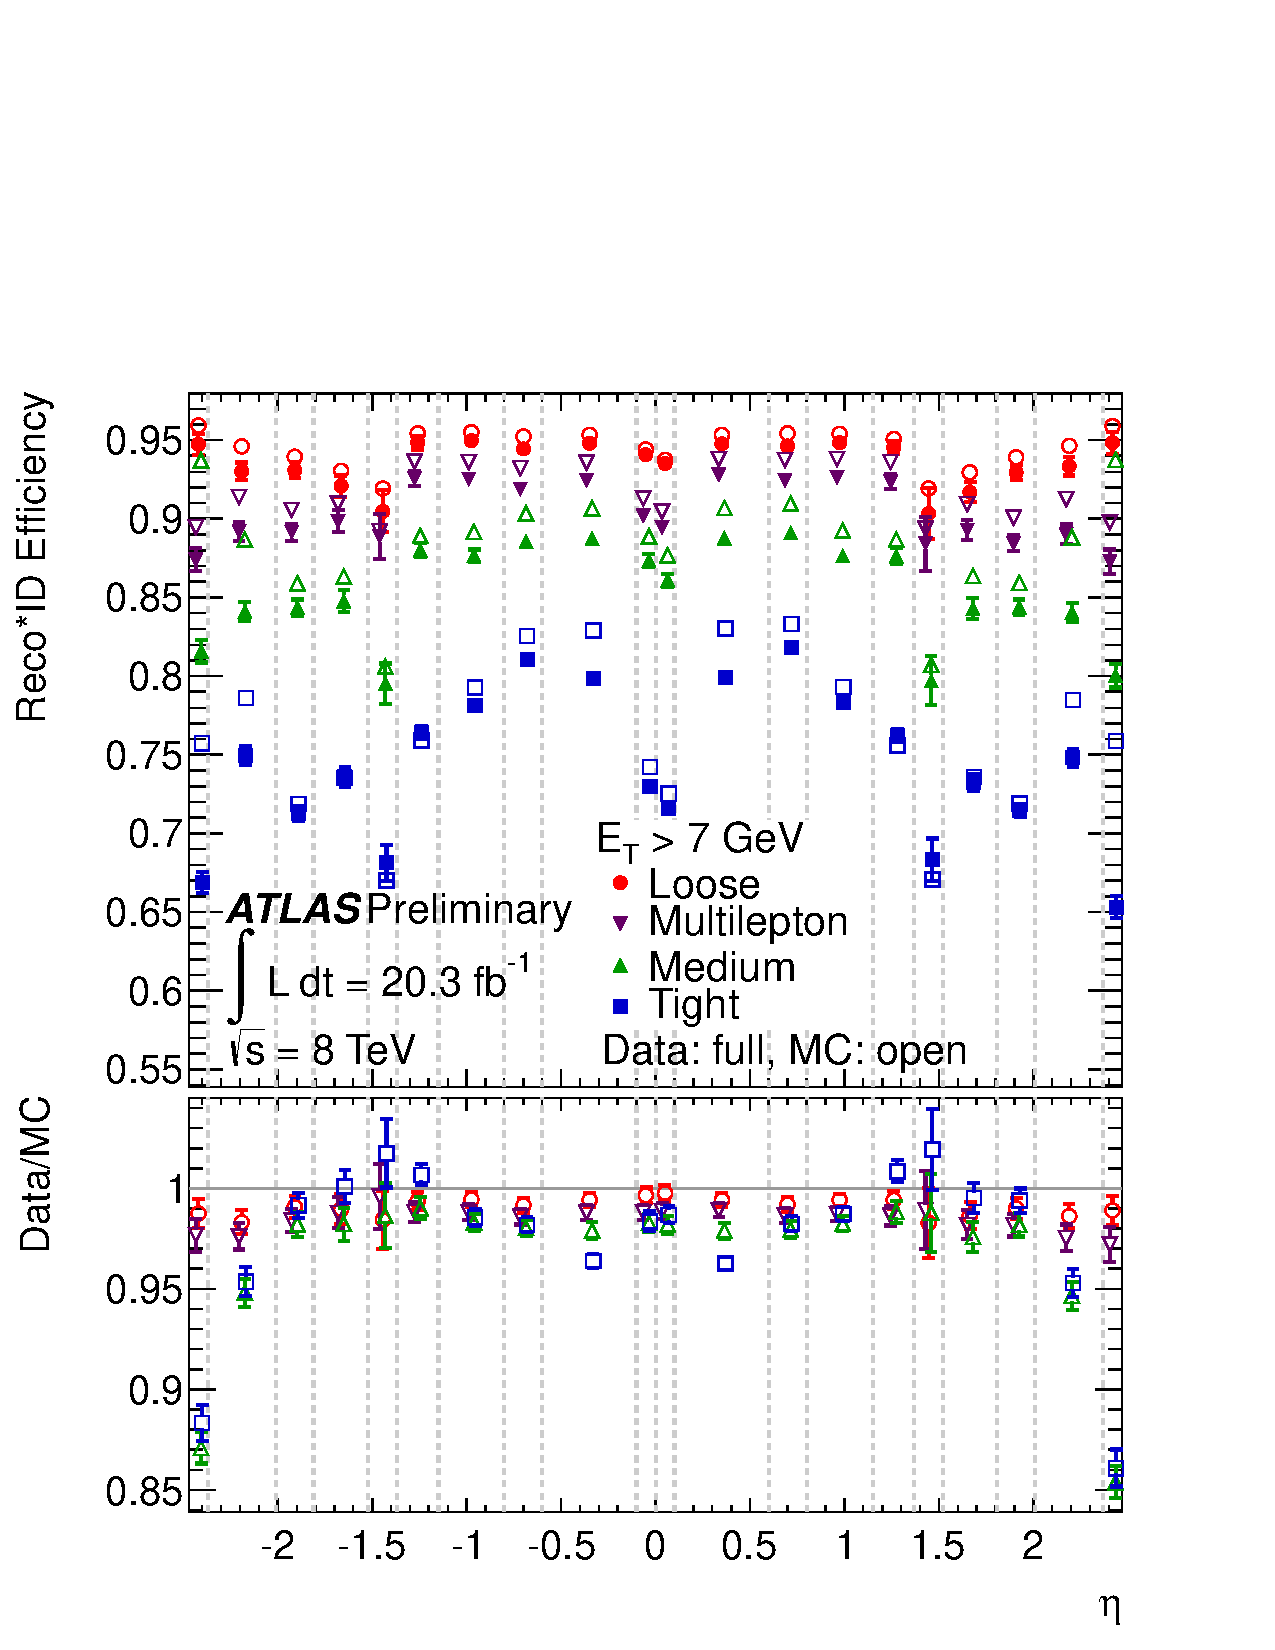
\includegraphics{figures/ch5-reconstruction/el_eff_idplusreco_eta}}
	}
	\caption{The combined reconstruction and identification efficiencies with respect to electrons detected as a cluster in the electromagnetic calorimeter, shown as a function of $\Et$ (left) and $\eta$ (right).}
	\label{fig:electron-id-efficiencies}
\end{figure}


\subsection{Energy and Momentum Measurement}\label{sec:reco-electron-energymomentum}
For electron candidates with at least four silicon hits, the energy of the electron is taken from the calorimeter measurement, while the trajectory is taken from the GSF track. Candidates with fewer silicon hits are not used in this dissertation. The energy resolution of the calorimeter is parametrized as:

\begin{equation}
	\frac{\sigma(E)}{E} = \frac{a}{\sqrt{e}} \oplus \frac{b}{E} \oplus c,
\end{equation}

where $a$, $b$, and $c$ are the sampling, noise, and constant terms, respectively, and generally vary with $\eta$. The design value of the sampling term is $a\approx 9-10\%$ in the central region, and worsens at higher pseudorapidities due to the increased material in front of the calorimeters. The noise term, due to electronics noise and pileup effects, is approximately $b = 350 \times \cosh\eta \MeV$. The constant term dominates the resolution at high energies, with a design value of $c=0.7\%$. 

As the ATLAS calorimeters are non-compensating, the energy measurement is calibrated using a multivariate algorithm trained on single-electron simulation to determine the most probable electron energy. The method takes into account differences between data and simulation in the energy scales of each longitudinal layer and other detector effects not modeled in simulation. 

After the initial simulation-based calibration, the electron energy scale and resolution are determined using $Z\rightarrow ee$ events. Residual differences in the energy scale between data and simulation are parametrized as:

\begin{equation}
	E^{\mathrm{data}} = E^{\mathrm{simulation}} (1 + \alpha_i),
\end{equation}

where the $\alpha_i$ quantify the energy scale difference in bins of pseudorapidity. The difference in energy resolution is derived assuming that the $Z\rightarrow ee$ invariant mass distribution is well-modeled up to a Gaussian constant term, 

\begin{equation}
	\left(\frac{\sigma_E}{E}\right)^{\mathrm{data}} = \left(\frac{\sigma_E}{E}\right)^{\mathrm{simulation}} \oplus c_i,
\end{equation}

where $i$ again denotes bins in pseudorapidity. Histograms of the $Z\rightarrow ee$ invariant mass distribution in simulation are then produced for a range of $\alpha_i$ and $c_i$ values, and the optimal values are determined using a $\chi^2$ minimization with respect to data. The results are shown in figures~\ref{fig:reco-el-EES} and \ref{fig:reco-el-EER}. 

Sources of systematic uncertainty on the energy scale include the intrinsic accuracy of the $Z\rightarrow ee$ method, determined from closure tests where known scale variations are injected into simulation, calorimeter gain and pedestal dependence, data-simulation differences in the calibration of the calorimeter layers, and the modeling of material in front of and within the calorimeter. The total uncertainty ranges from $0.03$-$0.22$\% for $\Et=40 \GeV$ and $0.27$-$2.25$\% for $\Et = 200 \GeV$, with larger uncertainties in the pseudorapidity range $1.37<|\eta|<1.82$ corresponding to the transition region between the barrel and the end-cap. 

The systematic uncertainty on the energy resolution less than $10\%$ for electrons with $\Et<50 \GeV$, and asymptotically approaches $\sim 40\%$ for high $\Et$. At low energies, the pileup contribution to the noise term, $b$, dominates the uncertainty; at higher energy, uncertainty is due to a mix of the sampling term, $a$, the pileup contribution to $b$, the modeling of material, and the intrinsic accuracy of the $Z\rightarrow ee$ method.


\section{Muons}\label{sec:event-reconstruction-muons}
Muons are identified by matching tracks in the muon spectrometer to tracks in the inner detector. The requirements differ based on the instrumentation available in the vicinity of the muon candidate. The analyses described here use \emph{combined} muons, consisting of tracks reconstructed independently in the inner detector and the muon spectrometer. The muon momentum is determined from a statistical combination of the two track's parameters and their corresponding covariance matrices. Combined muons have the highest purity, but suffer from a loss of acceptance near $\eta\sim 0$, where the muon spectrometer has gaps to accommodate services for the inner detector and calorimeters, and $1.1<\eta<1.3$, where some trajectories only pass through one muon station due to incomplete installation. The remaining categories are \emph{standalone} (SA) muons, consisting of a track ony in the muon spectrometer; \emph{segment-tagged} (ST) muons, consisting of an inner detector track and one or more track segments in the MDT or CSC chambers; and \emph{calorimeter-tagged} (CaloTag) muons, consisting of an inner detector track matched to a calorimeter energy deposit consistent with the passage of a muon. These categories recover efficiency in regions of the detector with less instrumentation at the cost of lower muon purity, and are not used in this dissertation. 

For all categories of muons, the inner detector track is required to have at least 1 pixel hit, at least 5 SCT hits, at most 2 pixel or SCT holes, and at least 9 TRT hits for $0.1<|\eta|<1.9$. Energy losses in the calorimeter due to ionization, bremsstrahlung, and electron pair production must also be taken into account. 

\subsection{Efficiency}\label{sec:reco-muon-efficiency}
The efficiency of the reconstructing CB muons is measured as:

\begin{equation}
	\epsilon(\mathrm{CB}) = \epsilon(\mathrm{CB}|\mathrm{ID}) \epsilon(\mathrm{ID}|\mathrm{MS}),
\end{equation}

where $\epsilon(\mathrm{CB}|\mathrm{ID})$ is the probability that a muon reconstructed as an inner detector track is also reconstructed as a CB muon, and $\epsilon(\mathrm{ID}|\mathrm{MS})\approx \epsilon(\mathrm{ID})$ is the probability that a muon with a track in the muon spectrometer, i.e. a CB or SA muon, is also reconstructed as an inner detector track. The latter approximation is made because $\epsilon(\mathrm{ID})$ is not directly accessible in data. 

The efficiencies are measured using tag-and-probe techniques similar to those described in section~\ref{sec:reco-electron-efficiency}, targeting $Z\rightarrow\mu\mu$ and $J/\Psi\rightarrow\mu\mu$ events. In this case, the tag muon is required to be a CB muon, and the probe muon is a CB or SA muon in the case of measuring $\epsilon(\mathrm{ID}|\mathrm{MS})$, and a CaloTag muon for the measurement of $\epsilon(\mathrm{CB}|\mathrm{ID})$. The efficiencies for all types of muon are shown in figure~\ref{fig:reco-muon-efficiency}. CB muons have an efficiency of greater than $97\%$ in most of the pseudorapidity range, except for significant inefficiencies due to gaps in the muon spectrometer in the ranges $|\eta|<0.1$ and $1.1<\eta<1.3$. The measured efficiencies in data and simulation agree to within $\sim2\%$, and the ratios in each pseudorapidity bin are used as scale factors to correct the efficiency in simulation. The systematic uncertainty on the scale factors is in the range $0.1$-$0.3\%$, rising near $|\eta|\sim 0$ and $|\eta|\sim 2.5$.

\begin{figure}[htbp]
	\centering
	Figure 3 from muon paper, and 5a
	\caption{Top: Muon reconstruction efficiencies as a function of $\eta$ for muons with $\pt>10 \GeV$. The uncertainty bars on the points indicate statistical uncertainties. Bottom: The ratio between the measured and simulated efficiencies, with the combination of statistical and systematic uncertainties indicated by the uncertainty bars.}
	\label{fig:reco-muon-efficiency}
\end{figure}


\subsection{Energy Scale and Resolution}\label{sec:reco-muon-energymomentum}
The muon momenta in simulation are scaled and smeared to match the momentum scale and resolution in data. The corrections are derived in bins of $\eta$ and $\phi$, with boundaries chosen to minimize the variation of the correction in each bin, and are applied separately to the transverse momenta measured by the inner detector (ID) and the muon spectrometer (MS). Specifically, the correction is implemented as:

\begin{equation}
	\pt^{\mathrm{Cor,Det}} = \frac{\pt^{\mathrm{MC,Det}} + \sum_{n=0}^1 s_n^{\mathrm{Det}(\eta,\phi)(\pt^{\mathrm{MC,Det}})^n}}{1+\sum_{m=0}^2 \Delta r_m^{\mathrm{Det}}(\eta,\phi)(\pt^{\mathrm{MC,Det}})^{m-1}g_m},
\end{equation}

where Det=ID or MS, the $\Delta r_m^{\mathrm{Det}}(\eta,\phi)$ parametrize the momentum resolution smearing, the $s_n^{\mathrm{Det}}(\eta,\phi)$ parametrize the scale corrections, and the $g_m$ are normally-distributed random variable with mean 0 and width 1\footnote{Note that this equation does not apply to cases where the resolution is data is better than that in simulation. In these cases, the resolution difference is included in the positive ID and MS variations, and the effect of the positive variation on the physical observables is symmetrized about the nominal value.}. The constant scale correction term, $s_0^{\mathrm{MS}}$, accounts for the difference between data and simulation in the energy lost by muons before reaching the muon spectrometer. $s_0^{\mathrm{ID}}$ is set to zero due to the negligible energy loss before the inner detector. The linear terms, $s_1^{\mathrm{ID,MS}}$, models discrepancies between data and simulation in the magnetic field integral and the radial dimension of the detector. The resolution corrections $\Delta r_m^{\mathrm{Det}}$ represent deviations from the resolution in data, which is parametrized empirically as:

\begin{equation}
	\frac{\sigma(\pt)}{\pt} = \frac{r_0}{\pt} \oplus r_1 \oplus r2\cdot\pt,
\end{equation}

where the $r_0$ term describes energy lost by muons as they traverse the material of the detector, the $r_1$ term describes multiple scattering, magnetic field inhomogeneities, and local radial displacements, and the $r_2$ term describes intrinsic resolution effects due to the spatial resolution of the hit measurements and residual misalignment. 

The corrections are derived from $J/\Psi\rightarrow\mu\mu$, $\Upsilon\rightarrow\mu\mu$, and $Z\rightarrow\mu\mu$ events using a template maximum likelihood fit, similar to that described in section~\ref{sec:reco-electron-energymomentum}. The effect of the corrections on the invariant mass distribution of $Z\rightarrow\mu\mu$ events is shown in figure~\ref{fig:reco-muon-momentum-corrections}, along with the total systematic uncertainty. \textcolor{red}{Consider showing the muon momentum resolution, figure 14.}

\begin{figure}
	Figure 10c
	\label{fig:reco-muon-momentum-corrections}
\end{figure}



\section{Tau Leptons}\label{sec:event-reconstruction-taus}
The signature of tau leptons is significantly more complex than electrons and muons due to the fact that they decay to a diverse set of final states. Tau leptons have a proper decay length of $87 \micron$, and therefore typically decay before reaching the active layers of the detector. The leading decay modes are shown in table~\ref{table:reco-tau-decays}. $35.2\%$ of tau leptons decay to an electron or muon plus two neutrinos. The remaining $64.8\%$ decay to hadrons plus a neutrino. The hadronic decay modes contain one charged pion in $72\%$ of the decays, and three charged pions in $22\%$ of the decays; the majority of the remainder contain one or more kaons. The hadronic decay modes also frequently contain neutral pions, with $78\%$ containing at least one neutral pion. 


\begin{table}[htbp]
	\centering
	\begin{tabular}{|l|c|}
		\hline
		Decay & Branching Fraction \\
		\hline
		$e^- \overline{\nu}_e \nu_{\tau}$ & $17.83 \pm 0.04$ \\
		\hline
		$\mu^- \overline{\nu}_{\mu} \nu_{\tau}$ & $17.41 \pm 0.04$ \\
		\hline
		$\pi^- \nu_{\tau}$ & $10.83 \pm 0.06$ \\
		\hline
		$\pi^- \pi^0 \nu_{\tau}$ & $25.52 \pm 0.09$ \\
		\hline
		$\pi^- \pi^0\pi^0\nu_{\tau}$ & $ 9.30 \pm 0.11$ \\
		\hline
		$\pi^-\pi^+\pi^-\nu_{\tau}$ & $9.31 \pm 0.06$ \\
		\hline
		$\pi^-\pi^+\pi^-\pi^0\nu_{\tau}$ & $4.62 \pm 0.06$ \\
		\hline
	\end{tabular}
	\caption{Leading branching fractions of the tau lepton to final states with leptons or pions. Most of the remaining decays are to final states with kaons. From~\cite{pdg-tau}.}
	\label{fig:reco-tau-decays}
\end{table}

In this dissertation, no effort is made to identify or reconstruct leptonic tau decays ($\tau_{\mathrm{lep}}$), regarding them only as electrons or muons plus missing transverse energy (see section~\ref{sec:reco-met}). Hadronic tau decays ($\tau_{\mathrm{had}}$) are identified using their visible decay products, namely the neutral and charged hadrons, which are collectively called $\tau_{\mathrm{had-vis}}$. The signature consists of a narrow jet with one or three tracks, called one-prong or three-prong decays, respectively. Up to two $\pi^0\rightarrow\gamma\gamma$ decays are also included. The reconstruction and identification proceeds as follows~\cite{TheATLASCollaboration:2014tga}:

\begin{itemize}
	\item Jets reconstructed using the anti-$k_t$ algorithm with a distance parameter of $R=0.4$, built from TopoClusters calibrated with a local hadronic calibration. Jets with $\pt>10 \GeV$ and $|\eta|<2.5$ are used as seeds for tau lepton candidates.
	\item For each jet seed, the tau vertex is chosen to be the primary vertex with the greatest $\sum \pt$ of tracks in the region $\Delta R <0.2$ of the jet seed. This vertex defines the $\tau_{\mathrm{had-vis}}$ direction, i.e. is used to determine the $\eta$ and $\phi$ of the tau candidate. 
	\item $\pi^0$ candidates, consisting of a pair clusters within $\Delta R<0.2$ of the tau candidate, are identified using a BDT-based algorithm. Up to two $\pi^0$s are considered.
	\item A multivariate algorithm based on boosted decision trees (BDTs) is used to discriminate hadronic tau decays from the backgrounds, primarily due to jets with low track multiplicity. The BDTs use many input variables describing the energy cluster, the spatial arrangement and energy of the tracks, and the neutral pions. Separate BDTs are trained for one-prong and three-prong tau decays, using simulated $Z\rightarrow\tau\tau$, $W\rightarrow \tau\nu$, and $Z'\rightarrow\tau\tau$ decays for signal and collision data samples for the background. Three working points with different identification efficiencies are defined, called loose, medium, and tight. The performance of the identification algorithms is shown in figure~\ref{fig:reco-tau-efficiency}, along with correction factors applied to simulated samples to equalize the efficiencies in simulation and real data. The correction factors are derived by measuring the efficiencies in data and simulation, using a tag-and-probe method targeting $Z\rightarrow\tau_{\mathrm{lep}}\tau_{\mathrm{had}}$ events.
	\item An additional BDT-based algorithm rejects one-prong tau candidates consistent with an electron. The most powerful discriminating variables are the ratio of high- to low-threshold TRT hits on the track and the ratio of energies deposited in the electromagnetic and hadronic calorimeters. The electron rejection power versus the tau efficiency, derived from simulated $Z\rightarrow ee$ events, is shown in figure~\ref{fig:reco-tau-electron-rejection-efficiency}.  
\end{itemize}

\begin{figure}
	\centering
	Figures 5 and 11a from tau paper.
	\label{fig:reco-tau-efficiency}
\end{figure}

\begin{figure}
	\centering
	Figure 9
	\caption{Electron rejection power versus 1-track $\tau_{\mathrm{had}}$ efficiency for the electron rejection BDT. }
	\label{fig:reco-tau-electron-rejection-efficiency}
\end{figure}

\subsection{Energy Scale and Resolution}\label{sec:reco-tau-energymomentum}
The hadronic tau reconstruction and identification are based on calorimeter cells calibrated at the local hadronic scale. Several corrections are applied to correct the energy to a tau-specific energy scale (TES). First, corrections are derived using simulated $Z\rightarrow\tau\tau$, $W\rightarrow\tau\nu$, and $Z'\rightarrow\tau\tau$ events, generated with \pythia8. These corrections are determined as a function of the reconstructed $\tau_{\mathrm{had-vis}}$ energy and pseudorapidity based on the medium identification working point. A small pseudorapidity correction, reaching up to $|\Delta\eta|=0.01$, corrects a bias due to underestimated cluster energies in poorly-instrumented regions of the calorimeter. To account for pileup, $90$-$420 \MeV$ per additional reconstructed vertex is subtracted from the reconstructed $\tau_{\mathrm{had-vis}}$ energy, depending on $\eta$. The simulated $\tau_{\mathrm{had-vis}}$ energy resolution after these corrections is shown in figure~\ref{fig:reco-tau-energy-resolution}, and ranges between about $20\%$ at very low energy to about $5\%$ above a few hundred GeV.

Finally, data-driven corrections and systematic uncertainties on the tau energy scale are derived using a \emph{deconvolution} method~\cite{ref-49-from-tau-paper}. The method combines the systematic uncertainties on the single-particle response of the calorimeters based on the well-known branching fractions of hadronically decaying taus. A TES correction of about $1\%$ is determined. Including additional systematic uncertainties covering the detector modeling, pileup, non-closure of the calibration method, and the hadronic shower model, the total TES uncertainty is $2-3\%$ for one-prong decays and $2-4\%$ for three-prong decays.


\section{Jets}\label{sec:reco-jets}


%\subsection{Efficiency}

\subsection{Energy Scale and Resolution}

\subsection{$B$-tagging}\label{sec:reco-bjets}

\section{Invisible Particles}\label{sec:reco-met}
